\documentclass[margin=3mm]{standalone}
\usepackage{tikz}

\begin{document}

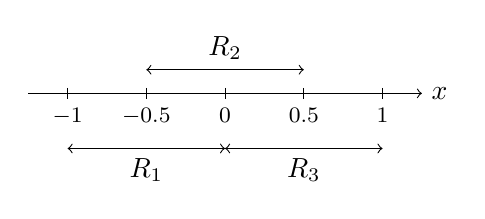
\begin{tikzpicture}
    \draw[->] (-2.5,0) -- (2.5,0) node[right] {$x$};
    \draw[distance=0.5mm,<->] (-2,-0.7) -- (0,-0.7) node[midway,below] {$R_{1}$};
    \draw[distance=0.5mm,<->] (-1,0.3) -- (1,0.3) node[midway,above] {$R_{2}$};
    \draw[distance=0.5mm,<->] (0,-0.7) -- (2,-0.7) node[midway,below] {$R_{3}$};
    \foreach \x in {-1,-0.5,0,0.5,1}
    \draw[shift={(2*\x,0)},color=black] (0pt,2pt) -- (0pt,-2pt) node[below] {\footnotesize $\x$};
\end{tikzpicture}

\end{document}